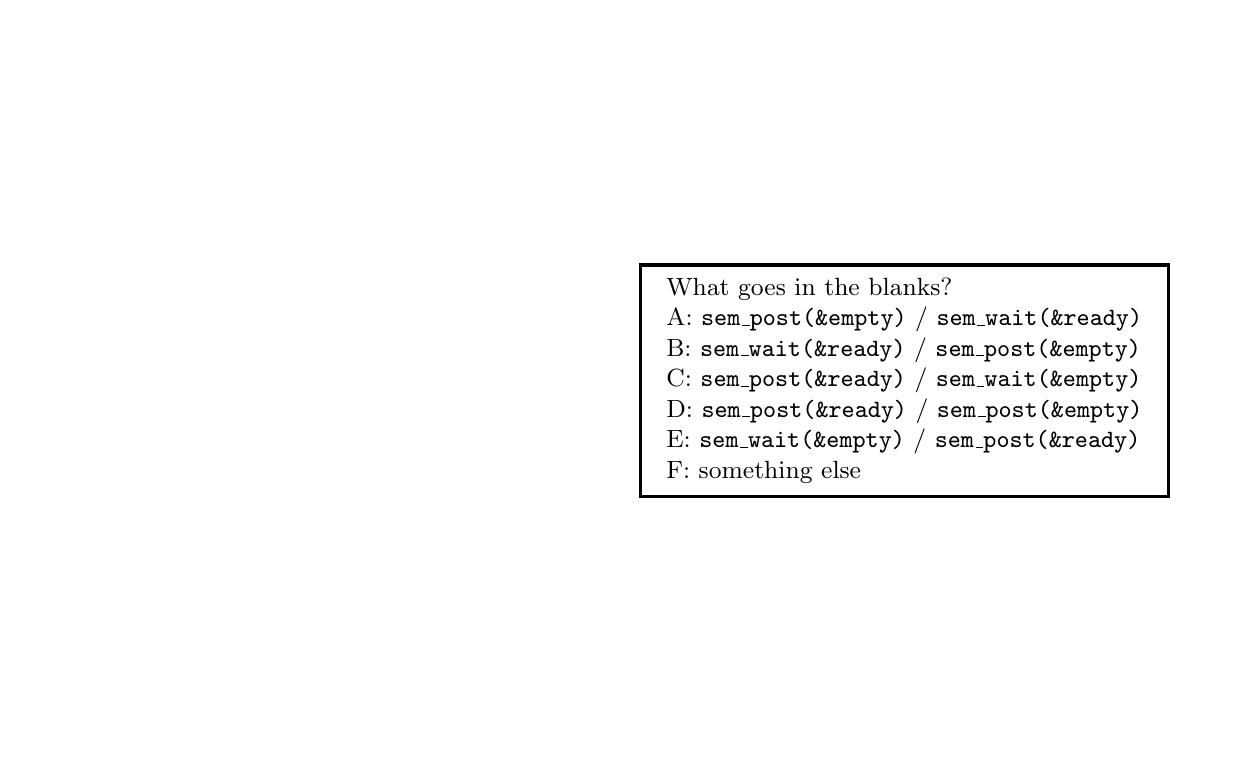
\begin{tikzpicture}
\node[minimum width=15cm,minimum height=9cm] (current page) {};
\begin{scope}[overlay]

\node[draw,very thick,anchor=north east,font=\small,fill=white] at ([xshift=-.5cm,yshift=-3cm]current page.north east) {
\begin{tabular}{l}
What goes in the blanks? \\
A: \texttt{sem\_post(\&empty)} / \texttt{sem\_wait(\&ready)} \\
B: \texttt{sem\_wait(\&ready)} / \texttt{sem\_post(\&empty)} \\
C: \texttt{sem\_post(\&ready)} / \texttt{sem\_wait(\&empty)} \\
D: \texttt{sem\_post(\&ready)} / \texttt{sem\_post(\&empty)} \\
E: \texttt{sem\_wait(\&empty)} / \texttt{sem\_post(\&ready)}  \\
F: something else \\
\end{tabular}
};
\end{scope}
\end{tikzpicture}
